\chapter{Dialog Systems}
\label{ch:03-dialog-systems}


\section{Using neural networks to generate dialog}
\label{ch:03-gen}

Sequence to sequence models are originally formulated to improve the automatic translation task [ref]. The authors of \cite{DBLP:journals/corr/VinyalsL15} proposed to use this model for generating dialog, and since then the field of dialog generation was revolutionized. As we have seen, a seq2seq model encodes the source sentence in a vector $\vect{h}$ and uses this vector to initiate a language model.

This can be used to model a dialog as follows: suposse we have recorded two agents A and B. We will use this dialog as the training data for our model. The model will try to predict how B would respond. Let $\vect{s} = s_1, s_2, \dots, s_n$ be an utterance from A and  $\vect{x} = x_1, x_2, \dots, x_m$ be the response from B (both $\vect{s}$ and $\vect{x}$ are a sequence of words). $\vect{s}$ is input to an encoder network, which is a RNN. The encodes summarizes the input utterance into a vector, say $\vect{h}$, and this vector is used to initiate the decoder model, which is another RNN. And the decoder takes as input $\vect{x}$ and at each time $t$ the model tries to predict the word $t+1$ using $x_1, x_2, ...., x_{t-1}, \vect{h}$. This became a multiclass classification task, and we train the model by minimizing the cross entropy loss.


After we training we can use the same model to generate a new dialog: the agent A gives an utterance ans we use the encoder model to summarize this uterance in a vector h as before, but now we use the probability distribution learned by the decoder model (initialized by $\vect{h}$) to sample words until it generates an end-of-speech <eos> token (or until a upper bound for the uterance size is reached). This approach allows for variable length inputs and outputs.

This is the base for more complex models. For example, take the hierarchical recurrent encoder-decoder architecture (HRED) proposed by Sordoni et al. \cite{Serban:2016a}. In this setting a dialogue is viewed as a sequence of utterances $D=\langle U_1 , \dots, U_M \rangle$ involving two interlocutors such that each $U_i$ contains a sequence of $N_i$ tokens, $U_i = \langle w_{i,1} , \dots, w_{i,N_{i}} \rangle$. Each $w_{i,j}$ is a random variable that taking values in the $V\cup A$ where $V$ is the vocabulary and $A$ is the set of \textit{speech acts} (for example 'pause' and 'end of turn' are  speech acts). In this case the learning task is the same as the one in language modeling: we want to estimate of the probability of one token (speech acts included) conditioned on the previously tokens:

\begin{equation}
P(w_{i,j} | w_{i,1}, \dots , w_{i,j-1}, U_{1}, \dots U_{i-1})
\end{equation}

The different dialogues $\langle U_1 , \dots, U_M \rangle$ will serve as a corpus.
In this paper the authors use a \textbf{Hierarchical Recurrent Encoder-Decoder model(HRED)}, i.e., a model based on three RNNs: an \textit{encoder} RNN, a \textit{context} RNN and a \textit{decoder} RNN.  To understand the workings of this model, suppose we have the following dialog:
\begin{itemize}
\item ($U_1$) Mom, I don't feel so good.\\
\item ($U_2$) What's wrong?\\
\item ($U_3$) I feel like I'm going to pass out.
\end{itemize}

First the encoder RNN will encode the sentence $U_1$ in a vector $\vect{U}_1$, then the context RNN will compute a hidden state, say $\vect{C_1}$ using $\vect{U}_1$ and all past sentences in the dialog. After that the decoder RNN will use $U_2$ as an input to predict the next word using $\vect{C_1}$. The same procedure is repeated for $U_2$. Figure
x shows the computational graph of this process.

\begin{figure}[ht!]
\label{HRED}
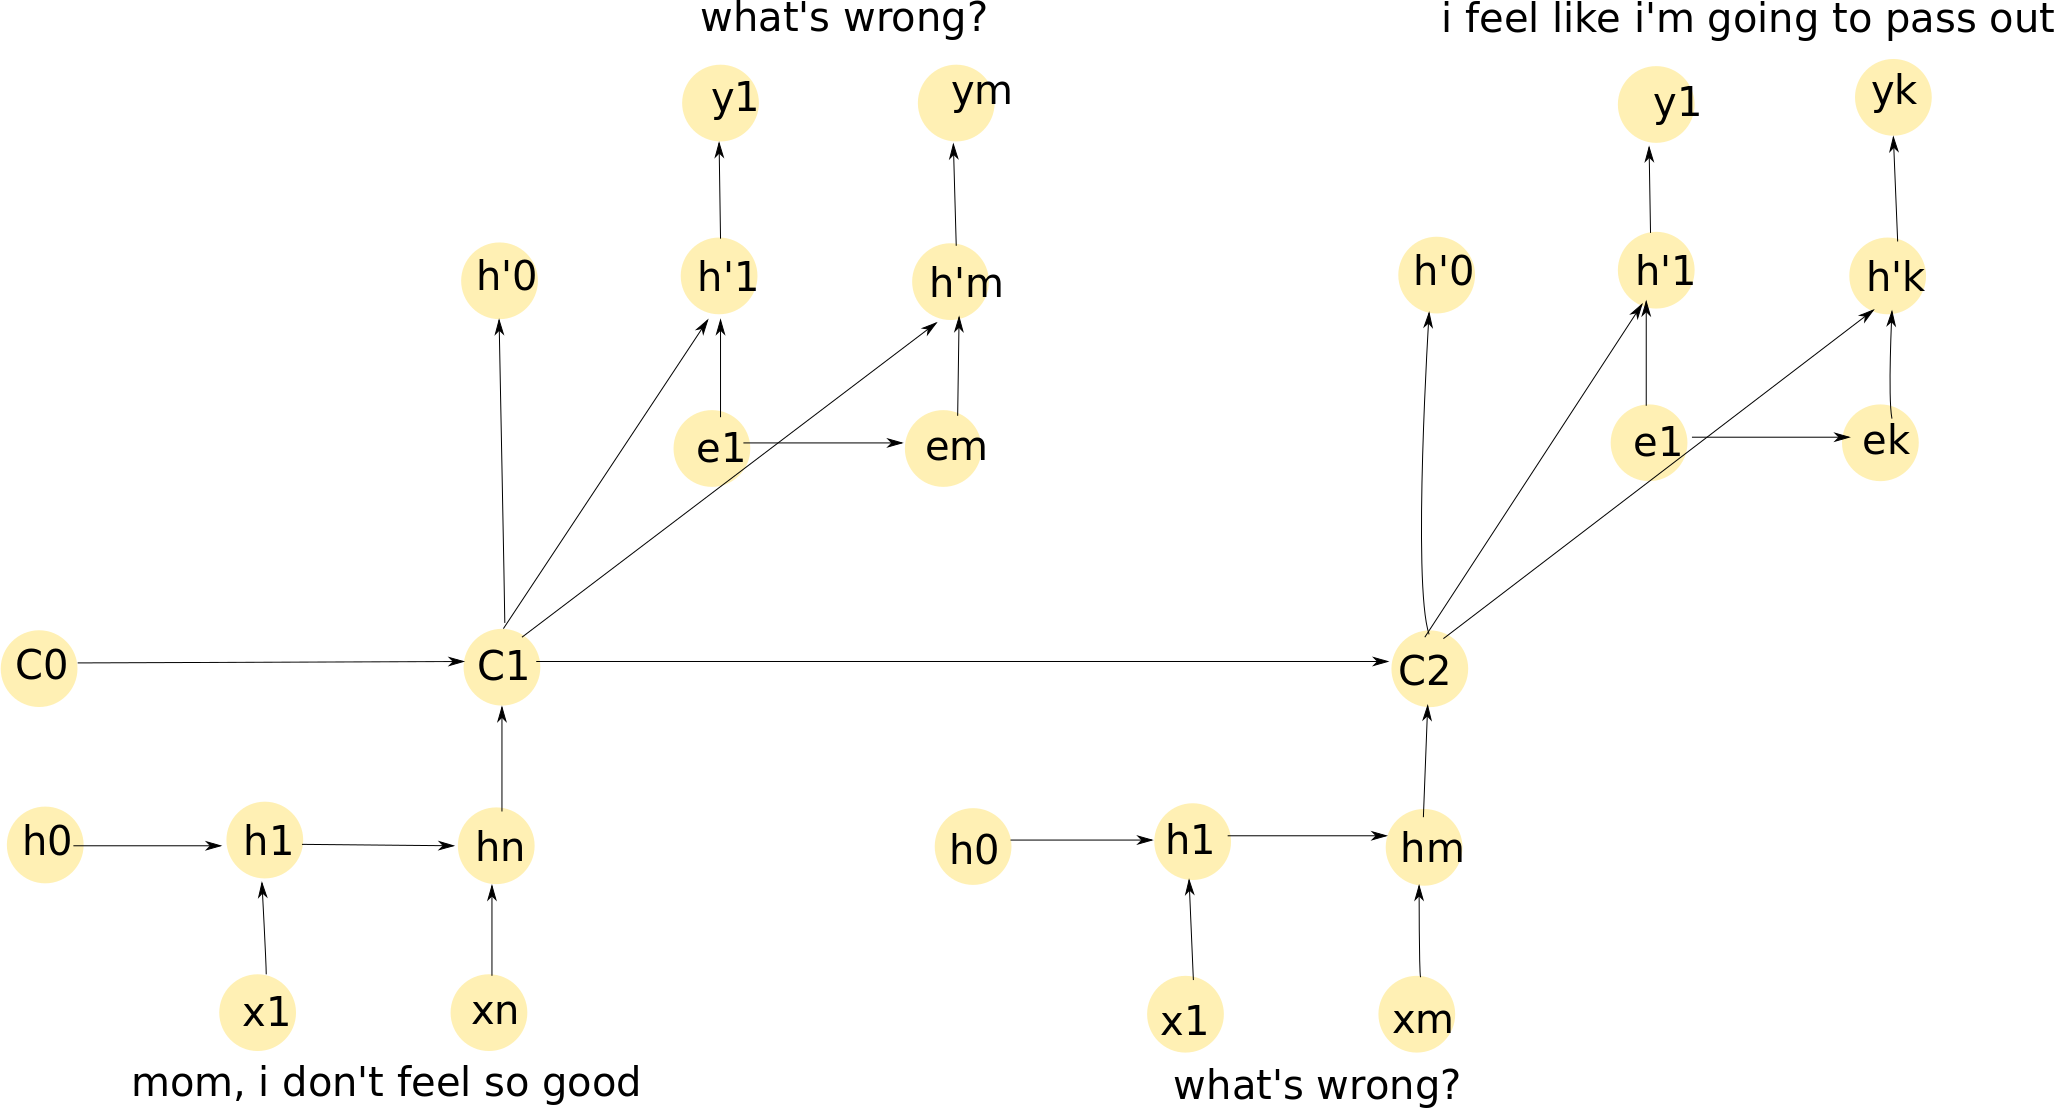
\includegraphics[width=10cm]{img/HRED_placeholder.png}
\caption{HRED model}
\end{figure}

Note that in this model the prediction is conditioned on the hidden state of the context RNN.



\section{How to evaluate dialogs?}

\label{ch:03-eval}

In the seminal paper by Alan Turing \cite{Turing} it is proposed a game to evaluate a dialog system. The idea behind the game was simple: three players A, B and C can interact only by nonpersonal communication. C knows that he will interact with a dialog system (A) and a person (B), but he does not know which is which. C should exchange some conversation both with A and B; after some time he should guess who is the dialog system and who is the human. The goal of A is to be as human as possible in order to fool C; and the goal of B is to help C come to the right answer.

\par This is the famous \textit{Turing Test}. If the dialog system wins this game we say that \textit{it has passed the Turing Test}. For many people this is the holy grail of artificial intelligence. We disagree with that. [Give your oppion about that]


\subsection{Human evaluation}

The most basic form to check if a generated sentence is sound is by using human evaluations. Hence is normal to see researches making use of crowdsourced judges (using services like Amazon Mechanical Turk). These judges can say that a generated sentence is just good or bad, in an informal way. But we can also use a more rigorous score system. 



In \cite{Stent} the authors enumerate three criteria to judge a generated sentence:

\begin{enumerate}
\item \textit{adequacy}: the meaning equivalence between the generated and control sentence. 
\item \textit{fluency}: the syntactic correctness of the generated sequence.
\item \textit{readability}: efficacy of the generated sentence in a particular context.
\end{enumerate}



\subsection{Automatic evaluation}


Because of the problems presented in using human judges, you can find in the literature the use of automatic metrics from the field of machine translation and automatic summarization.

\subsubsection{BLUE}



One popular metric for automatic translation is called BLUE (bilingual evaluation understudy) \cite{Papineni2001}. It compares n-grams of the candidate translation with the n-grams of the reference translation and counts the number of matches. Let $s$ be a source sentence $\hat{y}$ the hypothesis translation and $y$ a reference translations produced by a professional human translator. 

To define the BLUE score for each translation we need to define first the $n$-gram precision $p_n$:

\begin{equation*}
p_n = \frac{\text{number of } n\text{-grams in both } \hat{y} \text{ and } y}{\text{number of } n\text{-grams appearing in } \hat{y}}
\end{equation*}    

We also define a brevity penalty ($BP$) for translations that are too short. Let $len(a)$ be the length of the sentence $a$, we define $BP$ as:

\begin{equation*}
BP=
\begin{cases}
1 & \text{if } len(\hat{y}) > len(y) \\
\exp\left( 1 - \frac{len(y)}{len(\hat{y})} \right) & \text{otherwise}
\end{cases}
\end{equation*} 


Hence, the BLEU score is define as:

\begin{equation*}
BLEU = BP \; \exp \left(\frac{1}{N}  \sum_{n=1}^{N} \log p_n \right)
\end{equation*}

There are some details about the definition above: to avoid computing $\log 0$ all precisions are smoothed to ensure that they are positive (one technique of smoothing is to use a small positive value to replace any $p_n=0$); each $n$-gram in the candidate $\hat{y}$ is used at most once; and since its expensive to calculate higher $n$-grams we usually take $N=4$.

It is useful to see one application of this metric. For example, suppose $s$ is the Portuguese sentence `Nas tardes da fazenda há muito azul demais', $y$ is the reference English translation `In the farm's afternoons there is too much blue' and suppose we also have three models producing three distinct English translations 

\begin{itemize}
\item $\hat{y}_1$: `In the afternoons of the farm there is too much blue'
\item $\hat{y}_2$: `In the farm's afternoons there is a lot of blue'
\item $\hat{y}_3$: `The farm's afternoons are blue'
\end{itemize}


The table below shows all the values to compute the BLUE score for this example.

\begin{figure}[h]
\label{bluetable}
\begin{center}
\begin{tabular}{|c|c|c|c|c|c|c|}
\hline
\cellcolor{blue!10} Sentence & \cellcolor{blue!10} $p_1$ & \cellcolor{blue!10} $p_2$ & \cellcolor{blue!10} $p_3$ & \cellcolor{blue!10} $p_4$ & \cellcolor{blue!10} $BP$ & \cellcolor{blue!10} $BLUE$ \\ \hline
\cellcolor{blue!10} $\hat{y}_1$ & $8/11$ & $5/10$ & $3/9$ & $2/8$ & $1$ & $.42$\\ \hline
\cellcolor{blue!10} $\hat{y}_2$ & $7/10$ & $5/9$ & $4/8$ & $3/7$ & $1$ & $.52$\\ \hline
\cellcolor{blue!10} $\hat{y}_3$ & $3/5$ & $1/4$ & $0$ & $0$ & $.45$ & $.28$\\ \hline
\end{tabular}
\end{center}
\caption{Example of calculating $p_n$, $BP$ and $BLUE$ score}
\end{figure}

\subsubsection{METEOR}



The METEOR metric was created to address the weakness in BLUE \cite{Lavie}. This metric is based on an alignment between unigrams from the hypothesis translation $\hat{y}$ and unigrams from the reference translation $y$. This alignment can be based on exact matches, matching between stemmed unigrams, or matching by synonym.

After the alignment is done we compute the unigram precision $P$ and unigram recall $R$ as:

\begin{equation*}
P = \frac{\text{number of } \text{unigrams in both } \hat{y} \text{ and } y}{\text{number of } \text{unigrams appearing in } \hat{y}}
\end{equation*}    


\begin{equation*}
R = \frac{\text{number of } \text{unigrams in both } \hat{y} \text{ and } y}{\text{number of } \text{unigrams appearing in } y}
\end{equation*}    

We them combine these values using the harmonic mean:

\begin{equation*}
F_{mean} = \frac{10 P R}{R + 9P}
\end{equation*}

To take into account longer matches, this metric computes a penalty for the "chunkiness" of the alignment. The idea is to group the unigrams in fewest possible chunks. Here chunk is defined as a set of unigrams that are adjacent in $\hat{y}$ and in $y$. Hence the penalty is defined as

\begin{equation*}
penalty = 0.5 \left( \frac{c}{um} \right)^{3}
\end{equation*}

where $c$ is the number of $chunks$ and $um$ is the number of matched unigrams. Hence the METEOR score is defined as

\begin{equation*}
METEOR = F_{mean} (1 - penalty)
\end{equation*}

\subsubsection{ROUGE}

dkfskjdf


\subsection{The mismatch between human and automatic evaluation}



Table \ref{bluetable} shows the precision for each $n$-gram (up to $4$) and the BLUE score for each candidate.


 \cite{Stent}  page 7

\textit{Adequacy}: There  are  positive,  but  not  strong,  correlations  between  the  scores  of
the automatic evaluation metrics and human judgments of adequacy. We conclude that
these automatic evaluation metrics are adequate, but not good, evaluators of adequacy.

\textit{Fluency}: There are negative correlations between the scores of the automatic evalua-
tion metrics and human judgments of fluency. This is weakest in the case of LSA, which
does not consider word order. We conclude that (at least in the presence of variation)
these automatic evaluation metrics are poor evaluators of fluency



\section{Creating simplified tasks}
\label{ch:03-tasks}

Speak about bAbI


\section{The logical entailment problem inside the bAbI task}
\label{ch:03-tasks}


In \cite{WestonBCM15}, among a variety of useful tasks the authors introduce two tasks that deals with logical inference: \textit{basic deduction} and \textit{basic induction}. The basic deduction task offers questions of the form:

\begin{quote} 
\centering 
$P^{1}$ are afraid of $Q^{1}$\\
$P^{2}$ are afraid of $Q^{2}$\\
$P^{3}$ are afraid of $Q^{3}$\\
$P^{4}$ are afraid of $Q^{4}$\\
$c^{1}$ is a $P^{1}$\\
$c^{2}$ is a $P^{2}$\\
$c^{3}$ is a $P^{3}$\\
$c^{4}$ is a $P^{4}$\\
What is $c^j$ afraid of? A: $P^{j}$\\
\end{quote}

where $P^j$ and $Q^j$ are animals (e.g., "cats", "mice", "wolfs", etc.) and $c^j$ are names (e.g., "Jessica", "Gertrud", "Emily", etc.). The underlying relation under focus here is the \textit{membership} relation: if Emily is a cat and cats are afraid of wolfs then Emily is afraid of wolfs. This task is solvable by the current models, in \cite{WestonBCM15} the best accuracy for this task is $100\%$. 

The basic induction task is composed by questions of the form:

\begin{quote} 
\centering 
$c^{1}$ is a $P^{1}$\\
$c^{1}$ is $C^{1}$\\
$c^{2}$ is a $P^{2}$\\
$c^{2}$ is $C^{2}$\\
$c^{3}$ is a $P^{3}$\\
$c^{3}$ is $C^{3}$\\
$c^{4}$ is a $P^{4}$\\
$c^{4}$ is $C^{4}$\\
$c$ is a $P^{j}$\\
What color is $c$? A: $C^{j}$\\
\end{quote}

Where $P^{j}$ is a animal, $C^{j}$ is a color, and $c^{j}$ is a name. Here the agent is asked to remember the relation between animal and color, and when presented a new name of an animal in the example, the agent should infer the color using past examples. Similar to the deduction task, in \cite{WestonBCM15} is reported that this task is completely solved.

These two tasks present a first step towards \textit{a complete set of tasks to tests inference capabilities}. One aspect that is missing though is the use of logical operators such as \textit{boolean connectives} and \textit{first-order quantifiers}. Those operators play a big role on everyday speech, hence a natural way of expanding this work is by creating a set of tasks that make agents learn \textit{valid logic structures}.

\section{Entailment-QA}
\label{ch:03-EQA}

To highlight the speech structure we will make use of an artificial language, but, to be clear, this is just an exposition tool. We are concerned in logical structures \textit{only used in everyday speech}.

\textbf{Boolean Connectives} The first task is focused only on some propositional connectives $\land$ (and), $\lor$ (or), $\lnot$ (not). The agent is given two sentences $s_1$ and $s_2$, and he is asked if $s_1$ entails $s_2$ or not (a yes/no question). The position of the sentences is important here. We look at only six general cases:

\begin{itemize}
\item Entailment
\begin{itemize}
\item $\underbrace{P^{1}a^1 \land \dots \land P^{n}a^n}_{s_1}, \underbrace{P^{j}a^j}_{s_2}$ 
\item[]
\item $\underbrace{P^{j}a^j}_{s_1}, \underbrace{P^{1}a^1 \lor \dots \lor P^{n}a^n}_{s_2}$
\item[]
\item $\underbrace{Pa}_{s_1}, \underbrace{\lnot \lnot Pa}_{s_2}$
\end{itemize}
\item[]

\item Not entailment
\begin{itemize}
\item $\underbrace{P^{j}a^j}_{s_1}, \underbrace{P^{1}a^1 \land \dots \land P^{n}a^n}_{s_2}$
\item[]
\item $\underbrace{P^{1}a^1 \lor \dots \lor P^{n}a^n}_{s_1}, \underbrace{P^{j}a^j}_{s_2}$
\item[]
\item $\underbrace{Pa}_{s_1}, \underbrace{\lnot Pa}_{s_2}$
\end{itemize}
\end{itemize}

Where $P$ is a predicate and $a$ is a name. The point here is not to demand that the agent learn complex logical forms, but to recognize which forms are sound and which are not. This should be achieved independently from the content, i.e., the different predicates and names that appear on the sentences. So from the abstract forms above we have only simple examples like:

\begin{itemize} 
\item[] Ashley is fit
\item[] Ashley is not fit
\item[] The first sentence implies the second sentence? A: no
\end{itemize}

\vspace{0.3cm}


\begin{itemize} 
\item[]Avery is nice and Avery is obedient
\item[]Avery is nice
\item[]The first sentence implies the second sentence? A: yes
\end{itemize}

\vspace{0.3cm}

\begin{itemize} 
\item[]Elbert is handsome or Elbert is long
\item[]Elbert is handsome
\item[]The first sentence implies the second sentence? A: no
\end{itemize}

\textbf{First-Order Quantifiers} Task 2 tries to capture the use of some basic \textit{quantifiers}. In this dataset we are trying to predict the entailment relationship between two sentences $s_1$ and $s_2$. We say that there is a \textit{entailment} relationship if $s_1$ implies $s_2$, we say that there is a \textit{contradiction} if the combination of sentences $s_1$ and $s_2$ implies an absurdity and if the combination of sentences does not imply an absurdity we say that they are \textit{neutral}. We have used six forms of logical relations for the quantifiers $\forall$ (for every) and $\exists$ (exists):

\begin{itemize}
\item Entailment
\begin{itemize}
\item $\forall x Px, Pa$ 
\item $Pa, \exists x Px$ 
\end{itemize}
\item Contradiction
\begin{itemize}
\item $\forall x Px, \lnot Pa$ 
\item $\forall x Px, \exists x \lnot Px$ 
\end{itemize}
\item Neutral
\begin{itemize}
\item $Pa,Qa$
\item $\forall x Px, \lnot Qa$ 
\end{itemize}
\end{itemize}

where $P$ and $Q$ are non-related predicates and $a$ is a name. So we have examples like:

\begin{itemize} 
\item[] Every person is lively
\item[] Belden is lively
\item[] What is the semantic relation? A: entailment
\end{itemize}

\begin{itemize} 
\item[] Every person is short
\item[] There is one person that is not short
\item[] What is the semantic relation?  A: contradiction
\end{itemize}

\begin{itemize} 
\item[] Every person is beautiful
\item[] Abilene is not blue
\item[] What is the semantic relation? A: neutral
\end{itemize}


The tasks above force the dialog system to predict entailment independently of the specific meaning of nouns, verbs and adjectives presented on speech. To balance that we intend to design four more tasks centered on \textit{generic semantic knowledge}.

\textbf{Synonymy} This task tests if a dialog system can identify paraphrase caused by synonym use. Two supporting facts are presented, the second differs from the first by one noun, verb or adjective that can be a synonym or not, e.g., "\textit{The girl is talking into the microphone. The girl is speaking. Are the above sentences duplicate?}".   


\textbf{Antinomy} This task consists of recognizing contradictions by antinomy use. For example, the question "\textit{John is not an old person. John is young. Are the above sentences a contradiction?}" should be answered "no" and the question "\textit{Susan is happy. Susan is sad and she is crying. Are the above sentences a contradiction?}" should be answered "yes".

\textbf{Hypernymy} When one term is a specific instance of another we say that there is a hypernymy relationship between then. For example, we say that "anthem" is a hyponym and "song" a hypernym, because anthem is a kind of song. Task 5 tests the kind of linguistic entailment caused by the use of hyponyms and hypernyms, e.g., "\textit{A woman is eating an apple. A woman is eating a fruit. Are the above sentences duplicate?}"


\textbf{Active/Passive voice} Finally the last task is centered on the paraphrases originated by the changes from active to passive voice. So two supporting facts are presented, although they have a different syntactic structure, they share the same meaning. For example,  "\textit{A man is playing the piano. The piano is being played by a man. Are the above sentences duplicate?}".

It should be noted that we can formulate the notion of paraphrase as an entailment relation: if $s_1$ is a paraphrase of $s_2$, it is natural to say that $s_1$ implies $s_2$ and vice-versa. This is done in \cite{Marelli14}. Although this approach presents no problem it can alienate some people from the machine learning community: this community normally deals  with problems of similarity between sentences, there is very little datasets available centered on the notion of entailment. So although we have mentioned only paraphrase detection in tasks 3--6 the entailment relationship is present.


\section{Approach}
\label{ch:03-Approach}

% \cite{BordesW16, Lowe:2016, Serban:2016c, Serban:2016a,Shao:2017,Wen}

We will only consider \textit{neural network based end-to-end dialog systems}, these are the most important models today \cite{BordesW16, Lowe:2016, Serban:2016c, Serban:2016a, Shao:2017, Wen}. To organize all experiment in an unified framework we decided to use the platform ParlAI \cite{MillerFFLBBPW17}. Our criteria for a \textit{semantic robust dialog agent} is not an agent that is only tuned for the Entailment-QA tasks mentioned above, but an agent that performs well across all established tasks (like the bAbI tasks \cite{WestonBCM15}) and performs reasonably on the Entailment-QA tasks 1-6. Here "reasonably" means that the agent should exceed a random agent by a significant margin.

Right now we are in the process of creating the dataset. We have already built tasks 1 (boolean connectives) and 2 (first order quantifiers). They both are composed of 10000 questions for training and 1000 for testing.

We have used the dataset SICK (Sentence Involving Compositional Knowledge) \cite{Marelli14} as a proxy for tasks 3-6, since all the structures presented on those tasks are presented in this dataset. The SICK data is composed of a pairs of sentences and a label describing the entailment relation between the sentences. To cast this classification dataset as a question answering problem we have added a question and maintained the labels: 

\begin{itemize} 
\item[] A group of people are marching
\item[] A group of people are walking
\item[] What is the semantic relation? A: entailment
\end{itemize}

\begin{itemize} 
\item[] There is no dog leaping in the air
\item[] A dog is leaping high in the air and another is watching
\item[] What is the semantic relation? A: contradiction
\end{itemize}

\begin{itemize} 
\item[] A man is exercising
\item[] A baby is laughing
\item[] What is the semantic relation? A: neutral
\end{itemize}

\begin{itemize} 
\item[] Some dogs are playing in a river
\item[] Some dogs are playing in a stream
\item[] What is the semantic relation? A: entailment
\end{itemize}

This QA task is composed of 23000 questions for training and 5900 for testing.

\section{Preliminary results}
\label{ch:03-preliminary-results}

We have performed the first experiments using the sequence to sequence model \cite{Sustskever}(with and without attention: Seq2seq and Seq2seqAtt, respectively) and the memory network model (MenNN) \cite{WestonCB14}.

So far these models show unsatisfactory results, as can be seen in Figure 1.

\begin{center}
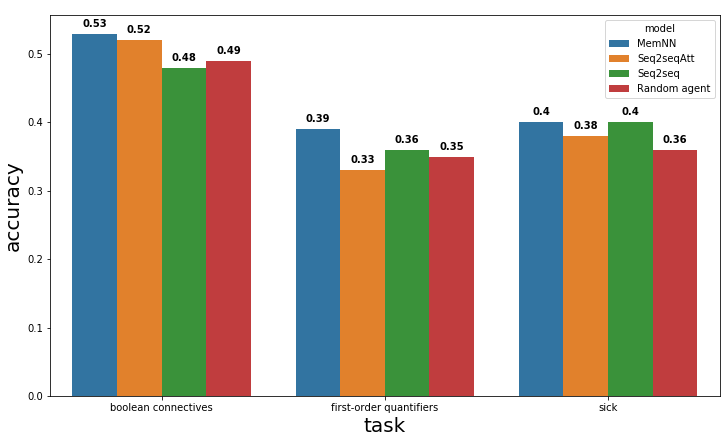
\includegraphics[width=10.0cm]{img/comparative_results.png}
% \captionof{figure}{Test accuracy for the Entailment-QA tasks}
\end{center}

Their overall performance is only slightly better when compared to the random agent. For example, when we look at the memory model, the model that often  outperform the seq2seq model on QA tasks \cite{WestonBCM15}, we can see that regarding tasks 1 and 2 there is an overfitting problem: the model shows high accuracy on the train dataset (75$\%$ accuracy on task 1, and 86$\%$ accuracy on task 2) as can be seen in Figure 2. But when we take a closer look at the confusion matrix of the test data, Figure 3, the results are not impressive.\footnote{All the experiments and the respective results are available on GitHub: \url{https://github.com/felipessalvatore/DialogGym}.}
  

\begin{center}
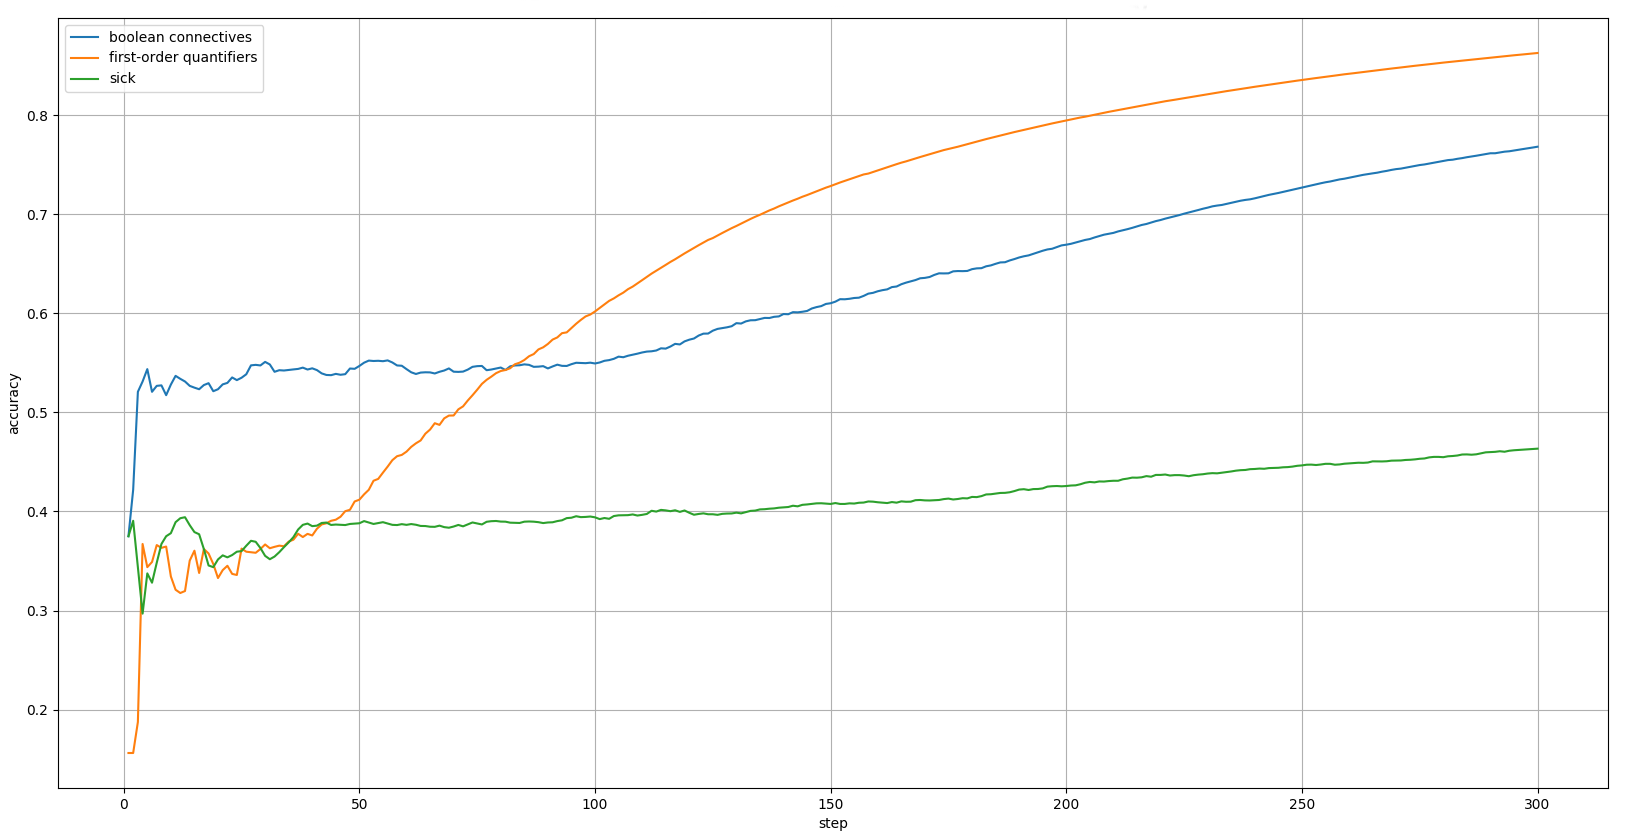
\includegraphics[width=10.0cm]{img/training_acc_EntailQA_mem.png}
% \captionof{figure}{Training accuracy for the memory network}
\end{center}


\begin{center}
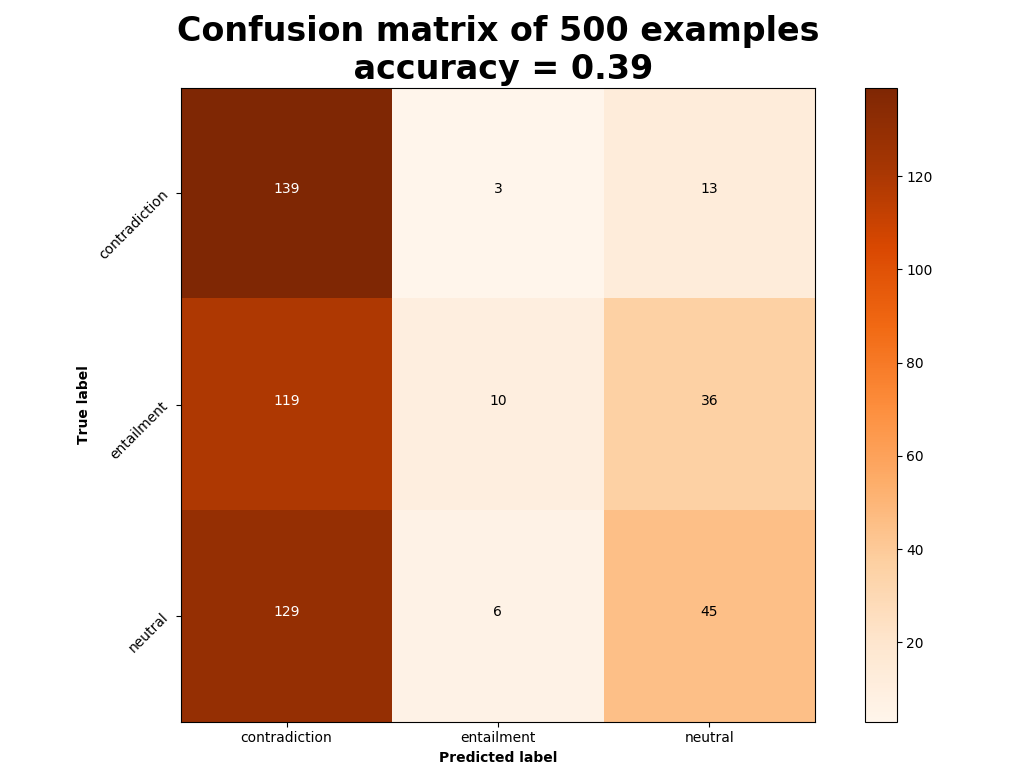
\includegraphics[width=10.0cm]{img/cm_mem_EntailQA2.png}
% \captionof{figure}{Confusion matrix for the memory network on task 2}
\end{center}


\section{KDD comments}
The paper presents a high quality and very interesting research. The concept of incorporating logic reasoning to boost performance of dialogue agent is very promising and employed by the authors in a novel way. The paper is focused on logical reasoning, the area that is often neglected by Conversational AI developers. Splitting the analysis for synonymy, antinomy, hypernymy and active or passive voice is hard to find in recent academic literature. These features make it an outstanding paper.

The Entailment-QA analysis of Neural Network dialog systems on 11000 questions provides interesting results. The fact that the overall accuracy is below 50$\%$ in many cases, points out a significant issue in the current phase of conversational AI. My only concern is that the methods of the research fall outside of Artificial Intelligence (AI) / Machine Learning (ML) domain which makes the paper less relevant to the workshop.

The paper is focused on specific issues of Conversation AI, in particular on complex semantic relationships. The paper is not covering machine learning aspects of Conversation AI. Instead the authors discuss a rule-based approach in more details. The paper would be a good fit for a workshop focused on rule-based methods in Conversational AI and for a workshop focused on automatic testing methods for chatbots. Due to the limitations on the number of accepted papers, this high quality paper might not make it to the short list. I would encourage the authors to proceed with their efforts to publish the paper elsewhere or come back next time when the workshop will have enough bandwidth.